\chapter{On-Body Device}
The on-body device was developed by William Tran in 2022~\cite{Tran:2022} and consists of two microcontrollers,
a PIC32 and a ESP32, as well as 24-bit ADC for taking biosignal measurements.

At the middle of the year when the project was handed over,
the ESP32 had been programmed to connect to WiFi, but was only programming intermittently,
and the PIC32 had bare-bones programming on it to enable the ESP32 via its enable pin.

The only other contributions were from Craig Dawson who supplied information and code for programming the PIC32,
as well as attaching wires to specific pins of the PIC32, allowing it to be probed using an oscilloscope.


\section{ESP32}
The ESP32 on the board is the ESP32-WROOM-32D.
This device is used as a wireless bridge between the on-body device and the off-body PC.
It connects to the PIC32 through a Serial Peripheral Interface (SPI) bus.
It is programmed using the Arduino software environment.

\subsection{Power}
As stated, the ESP32 was only programming intermittently.
To determine what the cause of this unwanted behavior was,
the board was tested in the following states in order to measure changes in how the ESP32 programmed.

\begin{itemize}
        \item The board was connected to a lab bench power supply with a non-restrictive current limit.
        \item The boot select switch was held for the extent of the programming cycle.
        \item The boot select switch was held until programming began.
        \item The boot select switch was held from when the device was powered on until programming ended.
        \item The board was powered from a lab bench power supply as well as via USB through an ICD 3.
        \item All the same boot select switch options were repeated with the additional power being supplied.
\end{itemize}

From this testing, it was discovered that the ESP32 programs successfully when it is being adequately powered
and the boot select switch is pressed as the device is being powered on.

The additional power requirement is not due to any external limitations with the lab power supply,
as the current draw that the supply is measuring is significantly less than the set current limit.
Additionally, there is a reduction in current draw from the first supply once the additional power supply is added.
This means that the load is being shared between the two supplies,
as opposed to the first supply being at its maximum output and the second supply providing necessary additional power.

What his means more broadly is that the problem with programming the device comes from the power distribution of the on-body device.
This can be further verified by measuring the voltage at points on the on-body device.
All of the ICs on the device operate at a 3.3V power level.
When measuring the voltage at the input pins of the ICs and at headers around the board, the voltage appears to be closer to 2.6V.
As we add additional voltage connections, we can observe the voltage rise.
Although the voltage does not reach 3.3V, the increase in voltage appears to be enough for the ICs to remain powered on.
This appears to be because the power traces on the board are not wide enough.
Because of this, the traces have significant resistance which causes a voltage drop to occur across them once the higher IC currents begin to flow.

For the ESP32, the lower voltage causes the brownout detection feature of the device to activate, causing it to reset.
% TODO: WEIRD SENTENCE RE-READ AND FIX MAYBE?
The effect that has on the device is that it will reset itself out of programming mode, causing the programming to fail.
This is because the ESP32 must be put into programming mode by holding down the boot select switch while the device is initially powered on.
So, even in instances when the device has been successfully put into this mode,
the device reset caused by the brownout detector reverts it out of this mode.

Once the power supply was supplemented with additional power supplies, this issue became less problematic.
However, additional issues arose as the ESP32 has to be placed into programming mode as it is powered.
With the addition of these power supplies, there is coordination required in order to get it into this mode.
Since the power is also required to keep the ESP32 from resetting, all of the supplies need to be disconnected and reconnected at the same time,
while the boot select switch is pressed.
Additionally, with this setup there is not way to validate the correct entry into programming mode,
meaning there is not way to know if it has actually been placed into the correct mode until the programming fails.
For prototyping, this becomes extremely cumbersome because this process must be repeated every time there is a change.
As well as whenever the programming fails due to an unexpected reset.

\subsection{Over-The-Air Programming}
Over-The-Air (OTA) programming is a technique used to program a device wirelessly~\cite{Quadri:2014}.
When compared to the alternative, OTA programming has a number of benefits.

\begin{itemize}
        \item The device can be programmed regardless of the boot mode.
        \item The device can be programmed without the use of a UART converter.
        \item The device can be programmed without a physical connection to a PC.
\end{itemize}

The downsides to this programming mode is that it adds additional compilation time, as well as minor overhead during run-time.
However, the compilation time is already in the range of 40 to 50 seconds, and the addition is less than 5 seconds,
and the run-time overhead can be mitigated by running OTA code in its own thread.
Considering these benefits and drawbacks, it was determined that this programming mode should be implemented.

The first step in implementing this feature was to connect the device to the network.
The ESP32 is programmed using the Arduino IDE, which contains a WiFi library for the ESP32.
The code for simple WiFi device bring-up is shown in~\autoref{code:wifi}.

\begin{lstlisting}[language=C++,caption={Arduino code for connected ESP32 to WiFi}\label{code:wifi}]
  #include <WiFi.h>

  void setup() {
    Serial.begin(115200);
    Serial.println('Booting');
    WiFi.mode(WIFI_STA);
    WiFi.begin(SSID, PASS);

    while (WiFi.waitForConnectResult() != WL_CONNECTED) {
      Serial.println(''Connection Failed! Rebooting...'');
      delay(5000);
      ESP.restart();
    }

  }
\end{lstlisting}

Once the device has been connected to the network, OTA programming can be implemented using the ArduinoOTA library.
This consists of including the ArduinoOTA.h header file,
configuring OTA updates using the code shown in~\autoref{code:ota},
and calling ArduinoOTA.handle() in the primary loop of the program.

\begin{lstlisting}[language=C++,caption={Arduino code for configuring OTA updates}\label{code:ota}]
  ArduinoOTA
  .onStart([]() {
    String type;

    if (ArduinoOTA.getCommand() == U_FLASH)
      type = `sketch';
    else // U_SPIFFS
      type = 'filesystem';

      Serial.println(`Start updating ' + type);
    })

    .onEnd([]() {
      Serial.println(`\nEnd');
    })

    .onProgress([](unsigned int progress, unsigned int total) {
      Serial.printf('Progress: \%u\%\%\\r', (progress / (total / 100)));
    })

    .onError([](ota_error_t error) {
      Serial.printf(`Error[\%u]: ', error);
      if (error == OTA_AUTH_ERROR) Serial.println(`Auth Failed');
      else if (error == OTA_BEGIN_ERROR) Serial.println('Begin Failed');
      else if (error == OTA_CONNECT_ERROR) Serial.println(`Connect Failed');
      else if (error == OTA_RECEIVE_ERROR) Serial.println('Receive Failed');
      else if (error == OTA_END_ERROR) Serial.println(`End Failed');
    });

\end{lstlisting}

After implementing these libraries, the ESP32 can be programmed using OTA by selecting the relevant device in the Arduino IDE.
One caveat of this is that the OTA updates will only be pushed as long as the OTA handler is called.
So, for instances where the ESP32 is in an infinite loop, or when there is a substantially long delay in the primary loop,
the ESP32 will need to be programmed using the original hardware method.


\section{PIC32}
The PIC32 on the board is the PIC32MX775F512H.
It connects to sensors, the 24-bit ADC, and the ESP32.
It is the main processor on the on-body device and it is programmed in C using MPLAB X v5.00 with an ICD 3.
The ICD 3 must be supplying 3.3V to on-body device in order for the PIC32 to be programmed successfully.

\subsection{Programming Configuration}
When the board was being manufactured, there was a global supply chain issue, as mentioned in Tran's thesis~\cite{Tran:2022}.
Because of this, the schematic design of the board was different to what was assembled on the board.
This caused issues when programming the PIC32, because the specific model of PIC had changed.
So, when the programmer connected to the device, it would read a different device ID from what was expected,
and the programming would fail.
Updating the project to use the PIC32MX775F512H solved this programming issue.

The other hurdle in programming the PIC32 was in the clock configuration.
With incorrect clock configuration, the device still programs, but it is not able to be put into debug mode.
Additionally, all delays that are added are based on the clock speed.
So it must be set correctly for the delays to be correct.

The clock configuration uses PLL~\cite{Maji:2016}.
It has been configured with a input divider of 10, a multiplier of 16, and an output divider of 8.
With a 16 MHz crystal, the system clock frequency becomes \((16 MHz / 10 * 16) / 8 = 3.2 MHz\).

The system clock frequency was verified by measuring the delay between pulses using an oscilloscope.
The code for delays in the system is shown in~\autoref{code:delay}, and code for generating output pulses is shown in~\autoref{code:pulses}

\begin{lstlisting}[language=C,caption={PIC32 code for adding delays in code execution (in microseconds)}\label{code:delay}]
  void delay_us(unsigned int us) {
    us *= DELAY_CONST;
    _CP0_SET_COUNT(0);
    while (us > _CP0_GET_COUNT());
  }

  void delay(int ms) {
    delay_us(ms * 1000);
  }
\end{lstlisting}

\begin{lstlisting}[language=C,caption={PIC32 code for measuring system clock speed using delayed pulses}\label{code:pulses}]
  #define TP7 PORTDbits.RD5 // Pin definition for test point 7

  void run() {
    TP7 = 1;
    delay(100);
    TP7 = 0;
    delay(100);
  }
\end{lstlisting}

The measured results for this are shown on the oscilloscope image seen in~\autoref{fig:pulse_delay}.
This figure shows a 100 ms delay between pulses.
This is exactly what the software delay has been set to, which verifies that the system clock frequency has been set correctly,
because the delay relies on the system frequency to calculate the desired amount of clock ticks to wait.
The equation for calculating the number of clock ticks is \(F_{sys} / 1000000 / 2\).
% TODO: MAYBE WHY AND WHERE THIS EQUATION HAS COME FROM? ALSO HOW THE DELAY NEEDS TO BE A CONST INSTEAD OF CALCULATED DUE TO OVERFLOW ERROR

\begin{figure}[!ht]
  \caption{Oscilloscope measurement of 100ms delay between pulses}\label{fig:pulse_delay}
  \centering
  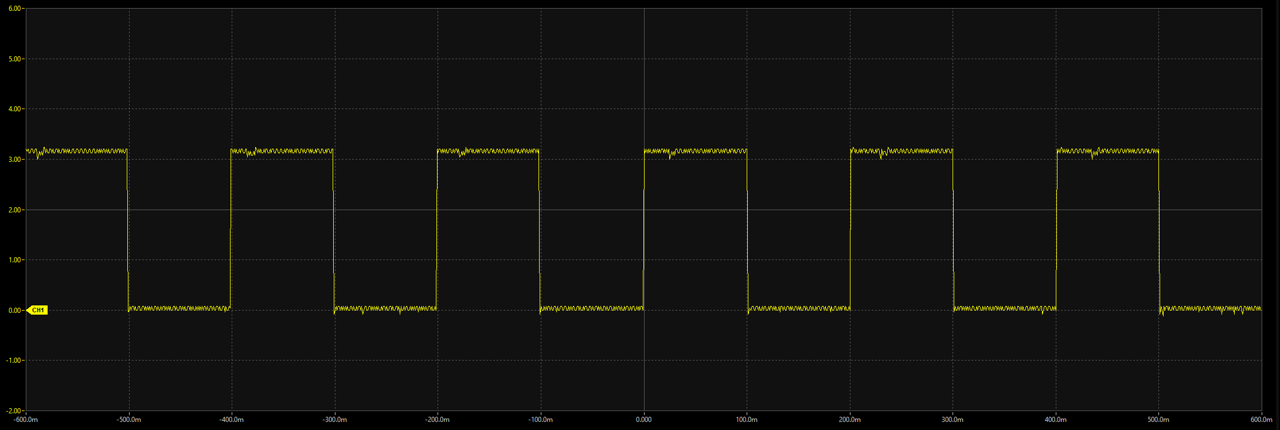
\includegraphics[width=1\columnwidth]{chapters/development/results/DELAY}
\end{figure}

With the system clock frequency set correctly, debugging works on the device and the CPU can be halted and stepped through instructions as the program is running.

\subsection{ESP32 Control}
The ESP32 is controlled by the PIC32 in two ways.

\begin{itemize}
        \item The ESP32 enable pin is connected to pin 14 (RB2) of the PIC32.
        \item The ESP32 HSPI bus is connected to SPI2 of the PIC32
\end{itemize}

The enable pin of the ESP32 just needs to be asserted high, which can be done by the PIC32 using the code shown in~\autoref{code:esp_en}

\begin{lstlisting}[language=C,caption={PIC32 code for enabling the ESP32}\label{code:esp_en}]
  void ESP32_IO_init() {
    TRISBbits.TRISB2 = 0;       // Set ESP32 EN pin as output
    PORTBbits.RB2 = 1;          // Set ESP32 EN pin high
  }
\end{lstlisting}

Without this assertion, the ESP32 is unresponsive to programming and does not perform code execution.

The other form of control is through the respective SPI lines of the two microcontrollers.
The SPI driver for the PIC32 is simple, as that device acts as the `master', which is the typical mode for a microcontroller to operate in.
The PIC32 is configured as a 32-bit master operating in SPI mode 3~\cite{Barry:2012}.
The baudrate generator value has been calculated using the equation \(BRG = (F_{PB} / 2 \times F_{SCK}) - 1\),
and a SPI clock speed of 31.3 kHz has been generated (using a BRG value of 50).
This value has been intentionally set low so that the transmission speeds are well below what both devices are capable of,
they can be easily raised by decreasing the value of BRG, once the system has been well tested.
Finally, the low-level SPI driver is implemented in~\autoref{code:spi_driver}

\begin{lstlisting}[language=C,caption={PIC32 low-level SPI driver}\label{code:spi_driver}]
  uint32_t ESP32_SPI_write(uint32_t data) {
    SPI2BUF = data;
    while(!SPI2STATbits.SPITBE);
    uint32_t read = SPI2BUF;

    delay_us(5000);
    return read;
  }
\end{lstlisting}

The function of the code is relatively straightforward.
The memory location of the SPI2BUF variable is mapped to the SPI 2 peripheral.
When written to, the data at this address is written into a transmit buffer that queues the data for SPI transmission.
When read from, data that has been received by the SPI peripheral is taken from the receive buffer.
Between these two operations the processor waits for the SPITBE status flag to be set.
This flag corresponds to the transmission buffer being empty, and is set once transmission has been completed and data has been received.

Additionally, a delay is required between SPI writes in order to stop data from becoming corrupt.
This delay was embedded into the low-level driver to make eventual performance optimization centralized,
since this delay is a clear cost to performance and by far the cause of the most communication slowdown.
This delay is most likely necessary due to the operation of the SPI chip select line.
Specifically, the way the chip select line does not reset between SPI transmissions without adequate delays between writes.
This could be solved by manually asserting the chip select line instead of allowing the peripheral to control it.
However, due to time restrictions it was decided that features should be implemented in a basic functional form,
and performance could be optimized once the system was fully functional.
and thus the driver was implemented using significantly slower delay.

The ESP32 SPI configuration was less straightforward.
As microcontrollers are typically the devices that coordinate communication between various `dumb' sensors,
they almost always act as the SPI master.
However, since the on-body device uses multiple microcontrollers communicating via SPI,
one of these devices needs to act as a slave.
Since the PIC32 is what communicates to the sensors, and the ESP32 only acts as a wireless transmitter,
the PIC32 was configured as the SPI master, leaving the ESP32 as an SPI slave.
There no official support for this in the native development environment, so a third party library was used.

The library that was used is the ESP32DMASPI library~\cite{ESP32DMASPI}.
This library is based on the official driver from the manufacture~\cite{SPI}.

SPI was implemented using task based DMA receiving.
In this setup, tasks run in separate threads, which frees up main thread to only process OTA updates.
One task runs continuously, waiting for SPI transmission~\autoref{code:esp_spi}.
% TODO: DESCRIBE IN MORE DETAIL HOW THESE WORK
%
\begin{lstlisting}[language=C++,caption={ESP32 code for receiving SPI data}\label{code:esp_spi}]
  void task_wait_spi(void* pvParameters) {
    while (1) {
      ulTaskNotifyTake(pdTRUE, portMAX_DELAY);
      slave.wait(buffer, BUFFER_LENGTH);
      xTaskNotifyGive(task_handle_process_buffer);
    }
  }
\end{lstlisting}

Once data has been received, a different task handles processing the incoming data~\autoref{code:esp_spi_processing}.

\begin{lstlisting}[language=C++,caption={ESP32 code for processing SPI data}\label{code:esp_spi_processing}]
  void task_process_buffer(void* pvParameters) {
    while (1) {
      ulTaskNotifyTake(pdTRUE, portMAX_DELAY);
      print_array(buffer, slave.available());
      slave.pop();
      xTaskNotifyGive(task_handle_wait_spi);
    }
  }
\end{lstlisting}

This should have been the end of the SPI implementation,
however the SPI communication did not work with just this code.
To get the communication working some additional functions were required on the PIC.
For example, the only way to send data was to write a single byte at a time, despite the fact that the SPI module is in 32-bit (4 byte) mode.
What is interesting about this is that the single byte must be located at the front of the 4 byte word.
This implies that the ESP32 was not able to receive 32-bits, and instead was just receiving the first 8-bit word.
However, if the SPI peripheral of the PIC32 was put into 8-bit mode (and all respective code changed to fit that mode),
the ESP32 would receive nothing.
So, the ESP32 required the PIC32 to send 32 SPI clock pulses but would only receive the first 8 data bits.
This same behavior was present when using both a task based approach or a polling approach and when DMA was or was not in use.
It is a substantial issue because it adds a 75\% overhead to the communication system.
This, and the required delay in the low-level driver, are the primary candidates for future optimizations.
The code for embedding data into a 4 byte word is shown in~\autoref{code:spi_additional_functions}.

\begin{lstlisting}[language=C++, caption={PIC32 additional SPI functions}\label{code:spi_additional_functions}]
  void ESP32_SPI_write_4byte(uint8_t b1, uint8_t b2, uint8_t b3, uint8_t b4) {
    uint32_t word = ((uint32_t)b1 << 24)
                  | ((uint32_t)b2 << 16)
                  | ((uint32_t)b3 << 8)
                  | (uint32_t)b4;

    ESP32_SPI_write(word);
  }

  void ESP32_SPI_write_byte(uint8_t data) {
    ESP32_SPI_write_4byte(data, 0, 0, 0);
  }
\end{lstlisting}

Despite significant performance issues, the drivers function together.
Allowing arbitrary bytes to be shared between the two devices.


\section{ADS1294R}
The ADS1294R is a 4 channel, 24-bit, delta-sigma analog-to-digital converter with additional features to support electrocardiogram and electroencephalogram measurements.
This device is the primary sensor front end.
It communicates with the PIC32 via SPI as well as several hardware control lines.

\subsection{Design Differences}
Like the PIC32, the schematic for the ADS1294R were slightly different to what was assembled due to chip shortages.
The schematic showed the devices as an ADS1298R, which is the 8 channel version of the device.
This is significant because the device requires a specific number of SPI clock pulses to be sent that correlates to the number of channels on the device.
So sending the wrong number of clock pulses will generate undesired results.
Additionally, the device ID is different which can cause some confusion when initially trying to configure the device.

\subsection{Startup Procedure}
The startup procedure of the device is shown in~\autoref{fig:ads_startup}.
When implementing this startup procedure, a similar SPI driver to what was seen in~\autoref{code:spi_driver} was used.
The key difference is that a higher delay was used for testing to ensure communication was well below data sheet limitations~\cite{ADS}.
When trying to follow this procedure, there were a number of key differences between what was expected and what was measured.
It appeared that no matter what command was sent, the response was always the binary number \(01100000\).
The data sheet specified responses for different registers, but regardless of the register the response was always the same.
The device also did not appear to respond to any two byte commands.
However, the device did respond to single byte commands.

\begin{figure}[!ht]
  \caption{ADS1294R startup sequence}\label{fig:ads_startup}
  \centering
  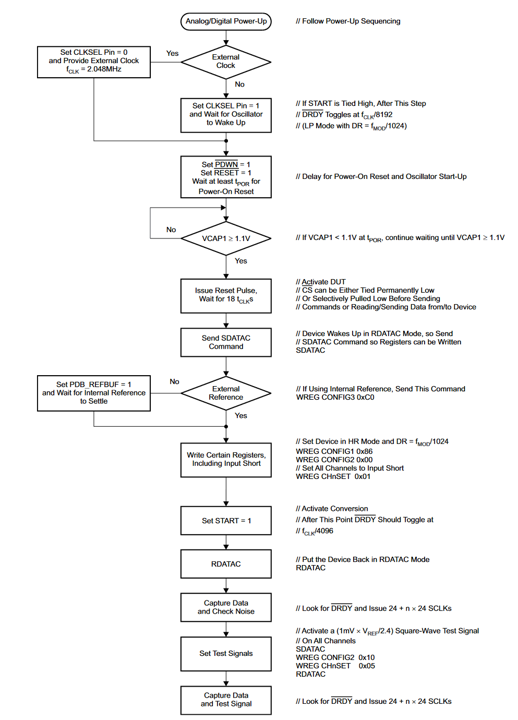
\includegraphics[width=1\columnwidth/2]{chapters/development/results/ADS_Startup_Sequence}
\end{figure}

The single byte commands were verified by monitoring the state of the data ready pin.
Since this pin was connected to the PIC and the PIC has general purpose test points on a number of pins;
the read value of the data ready pin can be written to one of the test points.
This effectively `passes through' the state of the pin.
The caveat being that any delays to the PIC will cause a delay between the data ready value and the test point.
As well as that it strips the signal of all information aside from if it has crossed the PIC's logic threshold.
However, the limited information it provides is still useful in this context.
Using an oscilloscope connected to the `pass through' test point, it is shown that the data ready pin is continually asserted.
This changes after calling single byte commands that change the state of the ADS1294R.
For example, if the reset command is continually send, the data ready pin will never be asserted,
once the command stops being sent, the data ready pin is reasserted.
Similarly, if the standby or stop commands are sent, the pin is not asserted until the respective wakeup or start commands are sent.
The exact same behavior is observed when the physical reset pin is held down, or when the start pin is asserted by the PIC.
What this says is that the device is powered and the transmit side of the SPI bus is connected correctly.
Since the SPI binary response is always \(01100000\), it can be assumed that the receive side of the SPI bus is also connected correctly.
This is because the response does not change and is both non-zero and also not continually driven high.
If either of those were true, the SPI bus could be picking up noise, or the receive pin may not be getting asserted.
But because of this response it must be being controlled by the ADS1294R SPI module,
since there is no other part of that device that is connected to the SPI clock and the response is the same even at higher and lower SPI clock speeds.

As the SPI hardware is assumed to be connected correctly, and the low-level SPI driver is confirmed to work with the ESP32,
the fault is assumed to be in the SPI configuration and startup procedure on the PIC.
Changing the clock polarity or clock phase causes the single byte commands to fail.
On top of that, changing the SPI interface off of 8-bit mode to 32-bit or 16-bit mode also caused the commands to fail.
The only change that could be made was the data sampling time, as this effected nothing to do with the transmission.
This change caused the received bits to change position,
but they were still not correct and different commands still caused the device to respond with the same response each time.
Therefore, the place in the program that was most widely explored was the code for the startup procedure.

The most obvious difference is that the startup procedure suggests using the hardware reset,
but that pin is tied to a physical switch instead of directly connected to the PIC.
Because of this, there is no way to automatically hardware reset the device in software,
so the reset has previously been achieved by sending the reset command.
To achieve a true hardware reset, a long delay was added to the startup sequence so that the physical switch could be pressed with the correct timing.
To aid with the timing, one of the test points was also driven high at the start of this timing window and low once the window had passed.
Then, using an oscilloscope to verify the timing window, the ADS1294R could be hardware reset at the correct point in the boot-up process.
This unfortunately did not solve the issue and the device still maintained the same issue as before.

Next, the register read and register write functions were investigated.
Since we had verified that the low-level driver was functional, and that same driver handled both the reading and writing,
it was unlikely that this was the issue, as this driver is so simple there are not many places errors could propagate.

The code for writing to the register is shown in~\autoref{code:ads_reg_write}.

\begin{lstlisting}[language=C, caption={PIC32 code for writing ADS1294R register}\label{code:ads_reg_write}]
  void write_register(uint8_t reg, uint8_t data) {
    static uint8_t write_register_cmd = 0x40;
    static uint8_t write_register_mask = 0x1F;

    uint8_t first_byte = write_register_cmd | (reg & write_register_mask);
    uint8_t second_byte = 0x00; // only ever write a single register

    ADS1294R_write(first_byte);
    ADS1294R_write(second_byte);
    ADS1294R_write(data);
  }
\end{lstlisting}

As the write commands were verified to be working, the changes to this function were around the register command byte,
register mask byte, and the addition of delays between writing the bytes.
However, these changes did not have any effect on the communication issues with the device.
We then turned our attention to the read register function shown in~\autoref{code:ads_reg_read}

\begin{lstlisting}[language=C, caption={PIC32 code for reading ADS1294R register}\label{code:ads_reg_read}]
  uint8_t read_register(uint8_t reg) {
    static uint8_t read_register_cmd = 0x20;
    static uint8_t read_register_mask = 0x1F;

    uint8_t first_byte = read_register_cmd | (reg & read_register_mask);
    uint8_t second_byte = 0x00; // only ever read a single register

    ADS1294R_write(first_byte);
    ADS1294R_write(second_byte);
    return ADS1294R_read();
  }
\end{lstlisting}

Similar changes and additions were added to this function, with the same result of the communication not working correctly.

At this point all of the command and register definition were double checked and
the register read and write functions were stepped through to verify that the bytes bit by bit, and all confirmed to be correct.

Since all logical software changes had been made and the system was still not functional,
it was decided that the SPI pins should be broken out so the communication could be analyzed using an oscilloscope.
Craig Dawson from engineering services helped in this aspect of the project,
since the pitch of the pins that needed to be soldered required specialized tools and expertise.
The device modifications are shown in~\autoref{fig:pic_wires}.

\begin{figure}[!ht]
  \caption{PIC32 board attached debugging wires}\label{fig:pic_wires}
  \centering
  \includegraphics[width=1\columnwidth]{chapters/development/results/P_20230919_170532}
\end{figure}


A four channel oscilloscope could then be used to analyze the SPI communication.
What was eventually discovered was that the chip select pin was not being asserted for long enough.
The SPI communication between the two devices is shown in~\autoref{fig:ads_spi}.
Since the chip select pin was being controlled by the PIC SPI module,
it was being automatically driven low during transmission and then high again after transmission completed.
This would have been the desired behavior, and it indeed was for single byte commands,
but for multi-byte commands the chip select line needed to stay asserted until all of the bytes had been transferred and received.

\begin{figure}[!ht]
  \caption{SPI communication between PIC32 and ADS1294R}\label{fig:ads_spi}
  \centering
  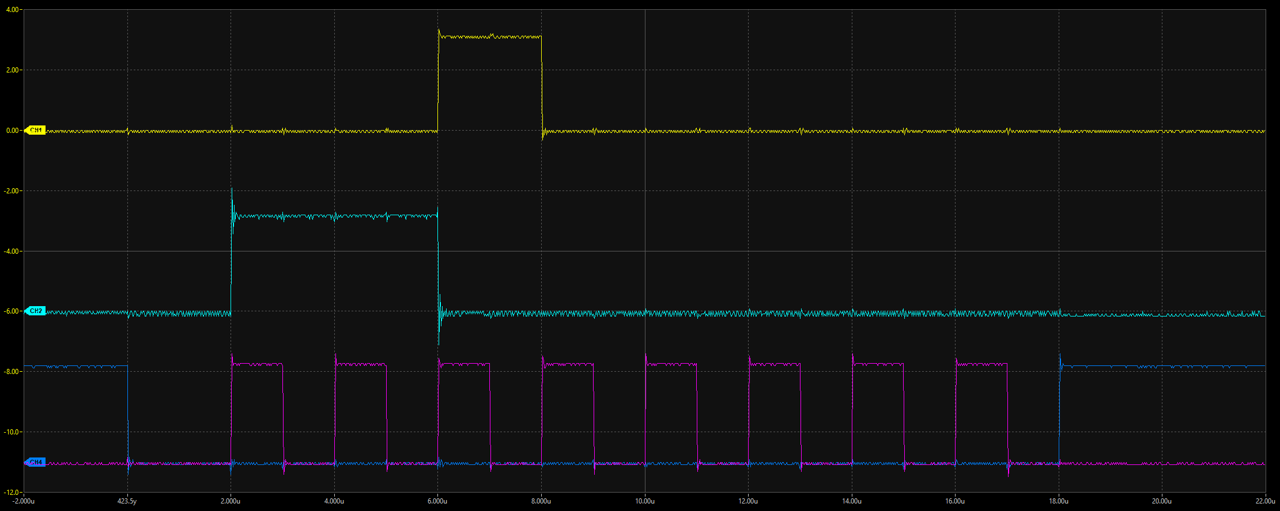
\includegraphics[width=1\columnwidth]{chapters/development/results/ADS_SPI_COMMS}
\end{figure}

The solution to this is to disable chip select control on the SPI module and manually set and reset the pin in software.
To accomplish this, the code was changed as shown in~\autoref{code:ads_cmd_write} and~\autoref{code:ads_updated_reg_funcs}

\begin{lstlisting}[language=C, caption={PIC32 code for writing single-byte commands to the ADS1294R}\label{code:ads_cmd_write}]
  void write_cmd(uint8_t cmd) {
    CS_PIN = 0;   // Chip select pin is active low
    ADS1294R_write(cmd);
    CS_PIN = 1;   // Chip select pin in inactive high
  }
\end{lstlisting}


\begin{lstlisting}[language=C, caption={PIC32 code for writing single-byte commands to the ADS1294R}\label{code:ads_updated_reg_funcs}]
  uint8_t read_register(uint8_t reg) {
    static uint8_t read_register_cmd = 0x20;
    static uint8_t read_register_mask = 0x1F;

    uint8_t first_byte = read_register_cmd | (reg & read_register_mask);
    uint8_t second_byte = 0x00; // only ever read a single register

    CS_PIN = 0;
    ADS1294R_write(first_byte);
    ADS1294R_write(second_byte);
    ADS1294R_read();
    uint8_t ret = ADS1294R_read();
    CS_PIN = 1;

    return ret;
  }

  void write_register(uint8_t reg, uint8_t data) {
    static uint8_t write_register_cmd = 0x40;
    static uint8_t write_register_mask = 0x1F;

    uint8_t first_byte = write_register_cmd | (reg & write_register_mask);
    uint8_t second_byte = 0x00; // only ever write a single register

    CS_PIN = 0;
    ADS1294R_write(first_byte);
    ADS1294R_write(second_byte);
    ADS1294R_write(data);
    CS_PIN = 1;
  }
\end{lstlisting}

With these changes, communication with the device is established and the device ID can be read successfully.
